
\chapter{Avaliação Experimental\label{sec:Avaliacao-Experimental}}

Este capítulo apresenta avaliação experimental da implementação da
arquitetura apresentada no capítulo \ref{sec:Arquitetura}. Os objetivos
gerais desta avaliação e a estruturação da mesma são apresentados
a seguir.

Na seção \ref{par:Hardwares-Testados}, foram realizados testes em
diferentes hardwares, permitindo avaliar sua capacidade de adaptabilidade
e compatibilidade tanto da perspectiva do middleware, quanto do firmware.
Na seção \ref{sec:Testes-de-Performance}, foram conduzidos testes
de performance com diferentes tecnologias de comunicação e protocolos,
permitindo avalizar a capacidade da arquitetura de lidar com tecnologias
heterogêneas e avaliar o desempenho e latências de comunicação. A
seção \ref{sec:Integracao3D}, apresenta experimentos de integração
com ambientes de desenvolvimento de jogos 3D (\emph{Game Engines}),
\emph{Blender} e \emph{jMonkeyEngine.} Estas ferramentas podem ser
utilizadas para criar ambientes de simulação, facilitando a criação
de aplicações de IoT, sem depender de um ambiente ou hardware real.
Por fim, a seção \ref{sec:Estudo-de-Caso}, apresenta um estudo de
caso, que permite avaliar a arquitetura proposta em um contexto real.
O contexto apresentado, está relacionado à automação residencial,
focando, principalmente, no controle de acesso usando a tecnologia
RFID.

\section{Hardwares Testados\label{par:Hardwares-Testados}}

Os testes realizados com os hardware estão subdivididos nas categorias
de microcontroladores (onde é executado o firmware) e os hardwares
na categoria de mini PCs que possuem um poder de processamento maior
e são destinados a executar o middleware ou aplicação construída utilizando
o framework.

\subsection{Microcontroladores (Firmware)}

Apesar do firmware ser construído com base na API do Arduino, o que
o tornaria automaticamente compatível com uma série de dispositivos
\cite{arduino-comp1,arduino-comp2,arduino-comp3}, os testes demostraram
que alguns microcontroladores possuem peculiaridades que têm que ser
levadas em consideração, principalmente pelo nível de abstração que
é proposto pelo sistema de configuração dinâmico de conexões que é
implementado (seção \ref{subsec:ConfiguracaoDinamica}). Como exemplo,
o firmware deve ser capaz de identificar quando estiver rodando em
um ESP8266, e realizar as configurações para conexão Wi-Fi sem necessidade
de modificações na aplicação/firmware.

A tabela \ref{tab:HardwaresTestados1} apresenta a lista de hardwares
dessa categoria que foram testados. Em seguida é apresentada a tabela
\ref{tab:HardwaresTestados1-mod}, com os módulos de conexão testados.

\begin{table}[h]
\begin{centering}
\begin{tabular}{|c|c|c|}
\hline 
Nome & Processador & Arquitetura\tabularnewline
\hline 
\hline 
Arduino UNO & ATmega328P - 16 MHz & AVR 8-bit\tabularnewline
\hline 
Arduino Nano & ATmega328P - 16 MHz & AVR 8-bit\tabularnewline
\hline 
Arduino Leonardo & ATmega32u4 - 16 MHz & AVR 8-bit\tabularnewline
\hline 
\textcolor{black}{Arduino MEGA} & ATmega2560 - 16 MHz & AVR 8-bit\tabularnewline
\hline 
Arduino Yun & ATmega32U4 / AR9331 Linux & AVR 8-bit\tabularnewline
\hline 
\textcolor{black}{Arduino Due} & ATSAM3X8E - 84 MHz & ARM 32-bit \tabularnewline
\hline 
ESP8266 & SoC (Tensilica's L106) - 80 MHz & RISC 32-bit\tabularnewline
\hline 
Stellaris Launchpad & LM4F120H5QR - 80 MHz & ARM M4F 32-bit \tabularnewline
\hline 
Digispark & ATtiny85 - 20MHz & AVR 8-bit\tabularnewline
\hline 
Teensy 3.1 & MK20DX256 - 72 MHz & ARM M4 32-bit\tabularnewline
\hline 
\end{tabular}
\par\end{centering}
\caption{Hardwares Testados (Microcontroladores)\label{tab:HardwaresTestados1}}
\end{table}

\begin{table}[h]
\begin{centering}
\begin{tabular}{|c|c|}
\hline 
Módulo & Conexão\tabularnewline
\hline 
\hline 
Arduino Ethernet Shield & Ethernet\tabularnewline
\hline 
Módulo ENC28J60 & Ethernet\tabularnewline
\hline 
ESP8266 (AT Mode) & Wi-Fi\tabularnewline
\hline 
HC-05 / HC-06 & Bluetooth SPP\tabularnewline
\hline 
\end{tabular}
\par\end{centering}
\caption{Hardwares Testados (Módulos)\label{tab:HardwaresTestados1-mod}}
\end{table}


\subsection{Mini PCs}

No trabalho, nomeamos de mini PCs, os hardware capazes de executar
um sistema operacional completo, como o Linux, e que possuem 512MB
de memória RAM ou superior. Hardwares baseados na arquitetura ARM
são elegíveis para suporte a máquina virtual Java (JVM), consequentemente
tendo suporte para execução do middleware. Entretanto a forma de acesso
aos periféricos dos mesmos, como os pinos de GPIO, são específicos
de cada plataforma. Não existe uma especificação genérica como a disponível
no framework do Arduino, que abstraia o acesso aos pinos de GPIO de
uma forma unificado. Uma proposta é API \emph{Device I/O}\cite{device-io:wiki},
porém, é um especificação nova e sua compatibilidade é limitada. 

\begin{table}[h]
\begin{centering}
\begin{tabular}{|c|c|c|}
\hline 
Nome & Arquitetura & RAM \tabularnewline
\hline 
\hline 
Raspberry Pi Model B (Alpha) & ARM & 256MB\tabularnewline
\hline 
BeagleBone Black & ARM & 512MB\tabularnewline
\hline 
\end{tabular}
\par\end{centering}
\caption{Hardwares Testados (Mini PCs)\label{tab:HardwaresTestados2}}
\end{table}


\section{Testes de Performance\label{sec:Testes-de-Performance}}

O objetivo deste experimento é avaliar a performance do middleware,
implementações das tecnologias de comunicação e do firmware.

\subsection{Procedimento de Medição}

Os experimentos foram executados através da ferramenta JMH\footnote{http://openjdk.java.net/projects/code-tools/jmh/},
que permite a criação de \emph{micro-benchmarks} em Java, isolando
alguns comportamentos da JVM, aproximando ao máximo de um ambiente
real. 

Os seguintes parâmetros de configuração foram utilizados na execução
dos testes:
\begin{itemize}
\item Iterações de pré-execução: 2;
\item Tempo de execução das iterações de pré-execução: 2s;
\item Iterações de coleta de dados: 20;
\item Tempo de cada iteração: 1s;
\item Argumentos da JVM: ``-server''.
\end{itemize}
As iterações de ``pré-execução'' são utilizadas para garantir que
a JVM, todas as classes da aplicação e bibliotecas, sejam carregadas
completamente, evitando interferência de acesso ao disco. 

Em cada iteração de coletas de dados são enviados um série de comandos
(\emph{DeviceCommand}) para os dispositivos, durante o período definido
(1s). Em cada iteração, são enviados o máximo de comandos possíveis
de forma sequencial e síncrona, permitindo calcular o tempo médio
de resposta de cada comando.

Ao final de todas iterações definidas (20), as estatísticas são geradas
pela ferramenta.

\subsection{Métrica Utilizada}

A métrica utilizada é o tempo de resposta fim-a-fim. Após todas iterações
serem executadas, é calculado o tempo médio de resposta de cada iteração
e em seguida, o tempo médio de reposta geral de todas iterações e
o erro médio.

O tempo de resposta, inclui o tempo para geração da mensagem no middleware,
transmissão, processamento e execução da ação no dispositivo e recebimento
da resposta.

\subsection{Resultados: Conexão USB}

\begin{figure}[H]
\begin{centering}
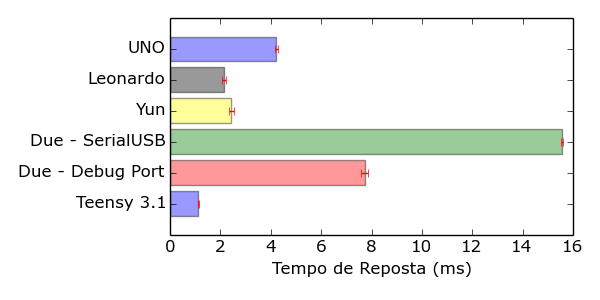
\includegraphics[width=0.8\linewidth]{Imagens/Cap_5/usb}
\par\end{centering}
\caption{Teste de performance - USB\label{fig:perf-usb}}
\end{figure}


\subsection{Resultados: Conexão Bluetooth}

\begin{figure}[H]
\begin{centering}
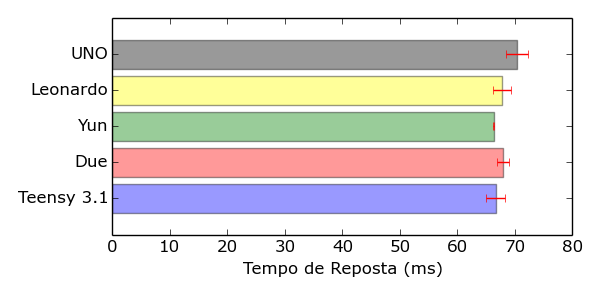
\includegraphics[width=0.8\linewidth]{Imagens/Cap_5/bluetooth}
\par\end{centering}
\caption{Teste de performance - Bluetooth\label{fig:perf-bluetooth}}
\end{figure}


\subsection{Resultados: Conexão Ethernet}

\begin{figure}[H]
\begin{centering}
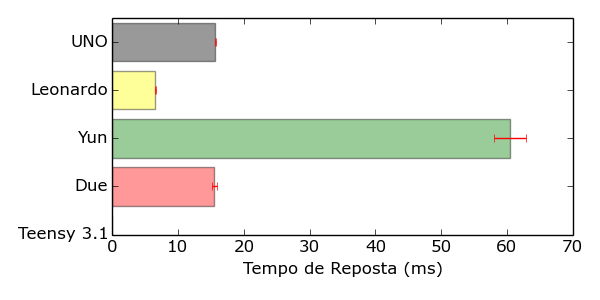
\includegraphics[width=0.8\linewidth]{Imagens/Cap_5/ethernet}
\par\end{centering}
\caption{Teste de performance - Ethernet\label{fig:perf-ethernet}}
\end{figure}


\section{Integração com Ambientes 3D\label{sec:Integracao3D}}

O desenvolvimento de aplicações para Internet das Coisas conta com
o desafio de ter que lidar com vários dispositivos físicos. Como alternativa
ambientes de simulação podem ser utilizados para executar os testes
e experimentos, antes de testar com os dispositivos reais. Outra possibilidade
para utilização dos ambientes 3D, é permitir a integração entre um
ambiente real e virtual.

Foram realizados testes de integração do OpenDevice com sistema de
desenvolvimento de jogos (\emph{Game Engine}), afim de validar uma
possível utilização dos mesmos para criação de ambientes de simulação.
Os experimentos realizados são detalhados a seguir.

\subsection{Integração - jMonkeyEngine.}

A \emph{jMonkeyEngine}\footnote{\emph{http://jmonkeyengine.org/}}
é uma ferramenta gratuita de código fonte aberto, utilizada para construção
de jogos 3D em Java. Possui uma boa documentação e ambiente de desenvolvimento
integrado. Devido sua implementação ser baseada na linguagem Java,
a integração com o OpenDevice se torna bastante simples e permite
a construção de uma aplicação de simulação que utiliza as APIs e módulos
do OpenDevice diretamente, sem a necessidade do middleware. 

No teste realizado, foi construída uma aplicação simples para validar
a integração, que consiste no mapeamento dos dispositivos físicos,
no caso 3 LEDs, e sua vinculação com objetos virtuais 3D da \emph{Game
Engine}. Ao clicar em algum objeto 3D, como os representados na figura
\ref{fig:jmonkey}, o OpenDevice localiza o dispositivo vinculado
e envia o comando para o acionamento do dispositivo físico.

\begin{figure}
\begin{centering}
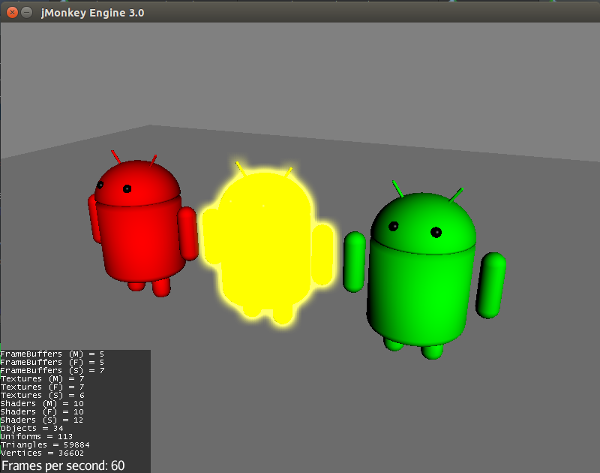
\includegraphics[width=0.8\linewidth]{Imagens/Cap_4/JMonkeyEngine}
\par\end{centering}
\caption{Integração com a JMonkeyEngine\label{fig:jmonkey}}
\end{figure}


\subsection{Integração - Blender.}

O \emph{Blender}\footnote{\emph{https://www.blender.org/}} é uma
ferramenta livre e de código fonte aberto, escrita em sua maior parte
utilizando a linguagem de programação Python. Ela possui ferramentas
para modelagem, animação, renderização e desenvolvimento de Jogos.
O diferencial em relação à \emph{jMonkeyEngine,} é que o \emph{Blender}
possui uma série de facilidades para configurações de eventos e vinculações
de scripts em Python utilizando apenas a interface gráfica.

Para permitir a integração com o OpenDevice, foi necessária a criação
de uma biblioteca cliente em Python, que implementa o protocolo do
OpenDevice e permite uma comunicação bidirecional através de uma comunicação
TCP. O experimento realizado (Figura \ref{fig:blender1}), é similar
ao experimento realizado com a \emph{jMonkeyEngine}, permitindo fazer
a vinculação entre objetos virtuais 3D e os dispositivos físicos\footnote{Vídeo do experimento da figura \ref{fig:blender1}: http://youtu.be/b3PbOPIMHmY}.

Para validar a performance da integração, foram realizados testes
visuais do tempo de resposta entre duas aplicações gráficas (Figura
\ref{fig:blender2}), uma escrita em Java (executando o middleware)
e outra Python. Verificou-se que as duas interfaces respondem em tempo
real às modificações na barra de rolagem (slider) em ambas interfaces\footnote{Vídeo do experimento da figura \ref{fig:blender2}: http://youtu.be/j4dMnAPZu70}.

\begin{figure}[h]
\begin{centering}
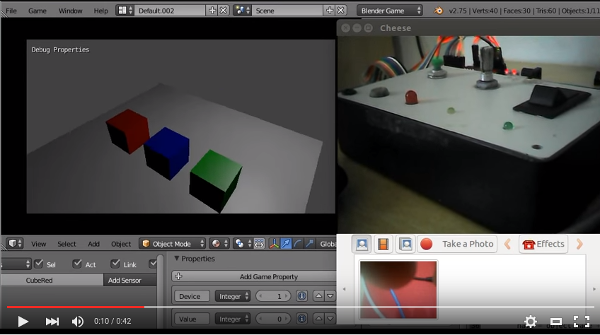
\includegraphics[width=1\linewidth]{Imagens/Cap_4/Blender}
\par\end{centering}
\caption{Integração com o Blender\label{fig:blender1}}
\end{figure}

\begin{figure}[h]
\begin{centering}
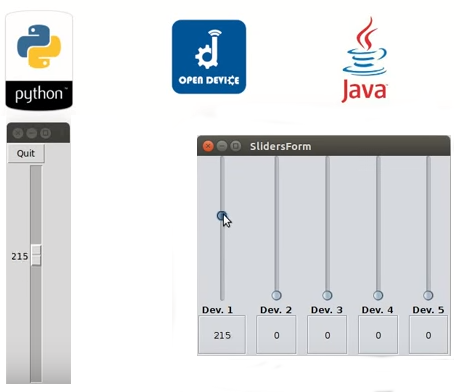
\includegraphics[width=0.7\linewidth]{/media/ricardo/Dados/Dropbox/Mestrado/Dissertacao/Imagens/Cap_4/Blender2}
\par\end{centering}
\caption{Teste de desempenho do cliente Python\label{fig:blender2}}
\end{figure}


\section{Estudo de Caso\label{sec:Estudo-de-Caso}}

A arquitetura descrita conforme a seção \ref{sec:Arquitetura}, foi
implementada vários testes foram conduzidos para validar os componentes
da arquitetura em relação ao design, integração e performance. Nesta
seção, faremos um estudo de caso baseado em um cenário real, permitindo
avaliar a integração entre os componentes da arquitetura e as capacidades
de evolução do framework proposto.

\subsection{Resumo}

O cenário escolhido para validação da proposta consiste em um sistema
de controle de acesso, usando a tecnologia RFID e alguns elementos
de automação residencial. A estratégia utilizada consiste na elaboração
de um cenário mais simples e sua posterior evolução para um cenário
mais complexo, integrando outros dispositivos e plataformas: Hardware,
Desktop, Web/Cloud e Mobile. O projeto será implantado nas instalações
do prédio denominado ``GEDAI'', onde está instalada a CriativaSoft
(empresa do autor) e outras duas empresas, sendo utilizado para o
controle de acesso dos funcionários. 

Os principais objetivos são: (1) avaliar os componentes da arquitetura
em conjunto, (2) validar os modelos de comunicação Cloud e Local,
(3) avaliar a integração com novos dispositivos (sensores e atuadores),
(4) avaliar a integração com dispositivos IP que utilizam outros protocolos,
(5) avaliar a integração com aplicações cliente Mobile(Android) e
(5) avaliar as capacidades de extensibilidade da plataforma.

\subsection{Ambiente de Teste}

Neste experimento serão utilizados hardwares de baixo custo, como
o Arduino, ESP8266 e Raspberry Pi, os demais sensores e atuadores
utilizados serão descritos nas seções seguintes. O middleware foi
implantado em um servidor na Amazon EC2, permitindo que aplicações
cliente controlem e recebam informações dos dispositivos pela Internet.

O experimento será avaliado em dois cenários, descritos e detalhados
a seguir.


\subsection{Cenário 1}

Este cenário tem como objetivo avalizar a utilização da arquitetura
do OpenDevice para criação de projetos simples para Internet das Coisas,
utilizando componente e hardwares existentes no mercado para criação
de projetos inovadores. Como mencionado, este cenário consiste na
criação de uma aplicação para controle de acesso usando RFID, conforme
apresentado na figura \ref{fig:cenario1}. Neste cenário, o hardware
está conectada à Internet através de uma comunicação Ethernet ou Wi-Fi
e se comunica com o middleware utilizando o protocolo do OpenDevice
em conjunto com o protocolo MQTT. Este cenário tem como característica
ser um cenário de fácil implantação. 

Para implementação dessa aplicação, foi utilizado o Arduino Yún, uma
versão do Arduino que possui conexão Ethernet e Wi-Fi já embutidas
na própria placa, e executa uma versão customizada no Linux para roteadores,
o OpenWrt-Yún\cite{openwrt-yun}, porém é possível utilizar qualquer
outra versão do Arduino, com um módulo que forneça uma comunicação
IP. A leitura dos cartões de acesso é feita por um leitor RFID de
proximidade que trabalha na frequência 13.56 MHz. O leitor é baseado
no processador MFRC522\cite{MFRC522} da empresa NXP, compatível com
cartões/tags RFID padrão ISO 14443A. A comunicação com este leitor
é realizada através do protocolo SPI\cite{spi1,spi2}.

\begin{figure}[H]
\begin{centering}
\includegraphics[width=1\linewidth]{Imagens/Cap_5/diagrama_caso1}
\par\end{centering}
\caption{Diagrama - Cenário 1 \label{fig:cenario1}}
\end{figure}


\subsubsection*{Estruturação do projeto:}

Neste cenário foram implementados duas aplicações: (1) uma aplicação
embarcada~(firmware), que faz o gerenciamento dos dispositivos físicos,
e (2) uma aplicação Java que utiliza o framework do OpenDevice, que
é a responsável pela validação dos cartões lidos. O firmware, utiliza
as bibliotecas do OpenDevice, MQTT\cite{lib-mqtt} e do leitor RFID
(MFRC522)\cite{lib-MFRC522}. A aplicação Java, é uma aplicação bem
simples, utilizando o módulo de servidor MQTT embarcado, o módulo
core da plataforma e um banco de dados em memória chamado MapDB\cite{mapdb},
com suporte a serialização em disco. O MapDB foi escolhido por ser
o mesmo utilizado na implementação do servidor MQTT (baseado no Moquette).

\subsubsection*{Descrição básica de funcionamento}

Ao detectar a presença de alguma etiqueta/cartão RFID, o firmware
envia a notificação para aplicação Java, que verifica a existência
do código lido no cache em memória (aumentando a performance) e envia
a resposta de confirmação de volta para o firmware, através de um
comando customizado (action), chamado \emph{``onAuthFinish}''. 

Na função ``\emph{onAuthFinish}'', definida pelo firmware, ele verifica
o parâmetro enviado pela aplicação, se a autenticação foi realizada,
em caso positivo, é emitido um sinal sonoro e liberado a fechadura
elétrica. Em caso negativo, é emitido um sinal sonoro longo e o acionamento
de um LED vermelho, permitindo o usuário identificar a não autorização.

O firmware conta com uma função que emite um alerta (sonoro e visual),
caso o servidor (aplicação Java) não efetue a resposta até um tempo
limite. É possível, também, a definição de chaves mestre, que não
necessitam de autenticação ``on-line'', permitindo a a liberação
do acesso caso não exista conectividade com a Internet.


\subsection{Cenário 2}

O cenário 2, representado pela figura \ref{fig:cenario2}, pode ser
considerado uma complementação do cenário 1, focado no controle de
acesso, mas incluindo novos elementos de automação. Neste cenário
é utilizado um servidor local, executando em um Raspberry Pi (ou BeagleBone),
e o mesmo está sincronizado com o middleware na Internet. 

O objetivo é avaliar o gerenciamento de vários dispositivos, a integração
com uma câmera IP (que opera com protocolo próprio), a interface entre
uma aplicação Mobile e dispositivos físicos pela Internet e a integração
entre uma aplicação local e o middleware instalado em um servidor
na nuvem.

Além do controle de acesso, usando RFID, este cenário integra uma
campainha sem fio, operando na frequência 433Mhz, uma câmera IP (clone
da Foscam) e um emissor de infra-vermelho para controle do ar-condicionado
da sala de reunião. 

\begin{figure}[H]
\begin{centering}
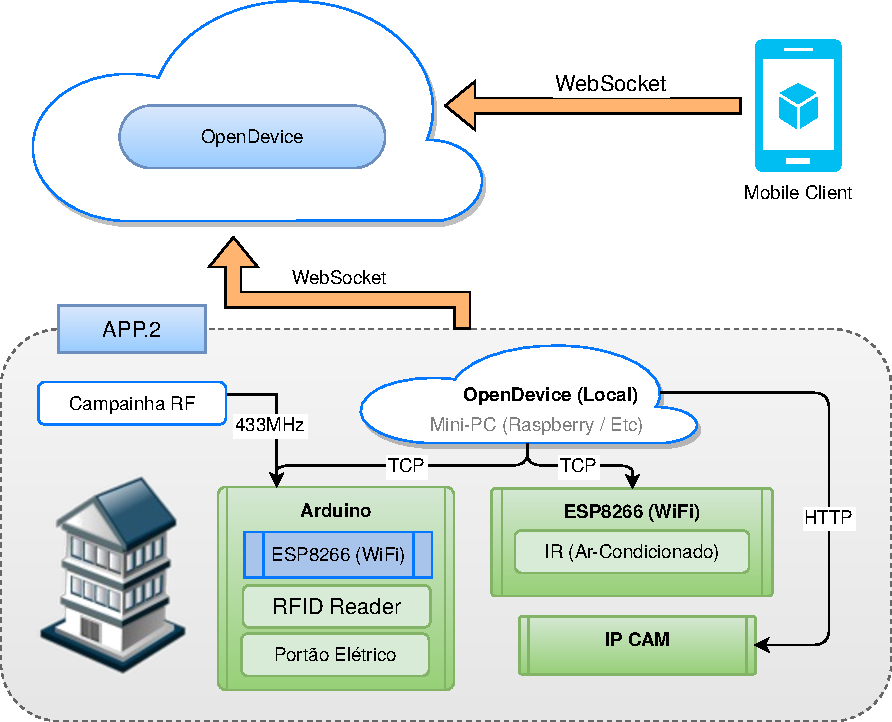
\includegraphics[width=1\linewidth]{Imagens/Cap_5/diagrama_caso2}
\par\end{centering}
\caption{Diagrama - Cenário 2 \label{fig:cenario2}}
\end{figure}


\subsubsection*{Descrição básica de funcionamento}

Quando a campainha é pressionada, o receptor RF 433Mhz acoplado ao
Arduino detecta o sinal e o firmware envia a notificação, via conexão
Wi-Fi, para a aplicação (ou middleware), que está executando no servidor
local. Em seguida, a aplicação captura a imagem da câmera IP e envia
uma notificação para as aplicações mobile, informando que uma visita
está aguardando a liberação, que pode ser realizada pelo próprio aplicativo
Mobile. 

\subsubsection*{Estruturação do projeto:}

Este cenário é composto por 5 aplicações/componentes, que serão detalhados
a seguir:
\begin{itemize}
\item \textbf{Dispositivo 1 (Arduino)}: Similar à implementação do cenário
1, com algumas modificações no hardware. Foi utilizado o Arduino UNO
e a conectividade Wi-Fi é fornecida pelo módulo ESP8266, utilizando
o firmware AT, conectado na porta UART do Arduino. Também foi incluído
um módulo receptor RF 433 Mhz que recebe o sinal da campainha. 
\item \textbf{Dispositivo 2 (ESP8266)}: O dispositivo que faz o controle
do ar-condicionado. Opera no modo independente (standalone), ou seja,
sem depender de outro componente. É programado com um firmware baseado
no framework do Arduino\cite{esp8266:arduino}, utilizando a biblioteca
do OpenDevice e a biblioteca para operar o emissor de infra-vermelho\footnote{https://github.com/markszabo/IRremoteESP8266}.
A comunicação com a aplicação local, é feita usando o protocolo MQTT
em conjunto com o protocolo do OpenDevice.
\item \textbf{Middleware Local}: Aplicação que executa localmente no Raspberry
Pi e responsável pelo gerenciamento de todos os dispositivos do projeto.
É baseada na versão padrão do middleware, e as regras específicas
para o projeto são implementadas através de extensões. As extensões
incluídas neste cenário adicionaram novas entidades persistentes,
novas interfaces Rest, suporte a novos dispositivos (câmera IP) e
novas páginas na interface administrativa do middleware. O sistema
de armazenamento utiliza a implementação padrão, baseada no Neo4J,
com suporte a JPA (Java Persistence API). A aplicação local possui
uma conexão com a versão do middleware que está implantado em um servidor
na nuvem (Amazon), permitindo que aplicações clientes controlem os
dispositivos pela Internet. 
\item \textbf{Middleware}: Implementação padrão disponibilizada pelo OpenDevice,
o middleware foi implantado em um servidor na nuvem, permitindo a
comunicação com dispositivos pela Internet, sem a necessidade de configurações
de IP Fixo ou DDNS (Dynamic DNS).
\item \textbf{Aplicação Mobile (Android)}: Permite a visualização da imagem~(posteriormente
vídeo) capturada pela câmera, liberação da fechadura elétrica e controle
do ar-condicionado da sala de reunião. A comunicação é realizada com
o middleware local, caso o dispositivo mobile esteja conectado na
mesma rede do middleware, ou com o middleware na Internet, caso esteja
usando uma rede 3G/4G.
\end{itemize}

\subsubsection*{Integração com Câmeras IP}

A câmera IP utilizada, utiliza um protocolo HTTP próprio. Para realizar
a integração, foi criado uma nova extensão que implementa a abstração
para este dispositivo. A extensão consiste basicamente na implementação
de duas classes: \emph{IPCamConnection} e \emph{IPCamGenericProtocol}. 

A classe \emph{IPCamGenericProtocol}, implementa a interface \emph{MessageSerializer},
é responsável por converter os comandos \emph{``ActionCommand}''
e \emph{``SetPropertyCommand}'', em requisições HTTP, seguindo as
especificações da câmera. O protocolo da câmera foi obtida através
de engenharia reversa e está disponível no website do autor\footnote{Protocolo câmera IP Foscam: https://goo.gl/yDUjDI}.


\section{Considerações Finais}

Este capítulo apresentou uma avaliação experimental, que abordou vários
aspectos e componentes da arquitetura proposta. Os testes de performance,
permitiram analisar a sobrecarga no tempo de comunicação com os dispositivos,
introduzido pelos componentes da arquitetura. Bons resultados foram
obtidos, principalmente na comunicação USB, mesmo sem a arquitetura
ter passado por nenhum processo de otimização.

Os experimentos conduzidos na seção \ref{sec:Integracao3D}, permitiram
avaliar positivamente, a possibilidade de integração com plataformas
3D, que podem ser usadas para criar ambientes de simulação.

Os experimentos realizados no estudo de caso (seção \ref{sec:Estudo-de-Caso}),
permitiram avaliar um amplo conjunto de componentes da plataforma.
O estudo de caso, cenário 1, permitiu avaliar a plataforma como framework
e a facilidade de implementação de projetos simples. O Cenário 2,
permitiu avaliar as capacidades de extensibilidade do middleware,
integração com vários dispositivos, utilização de várias tecnologias
de comunicação e hardwares. A integração com a câmera IP, apresentou
um real desafio, pois ela opera usando um protocolo próprio e é um
dispositivo relativamente complexo, pois possui controle de movimentação,
infra-vermelho, controle de brilho, saturação, tira fotos (snapshot),
vídeo e etc. Porém a integração foi bem sucedida, de modo que a câmera
e suas propriedades são totalmente acessíveis também da camada JavaScript
/ Web.

Estes experimentos demonstraram o potencial e flexibilidade da arquitetura
proposta.
